\documentclass[11pt]{book}
\usepackage[utf8]{inputenc}	% Para caracteres en español

\usepackage[left=2.75cm,right=2.75cm,top=2cm,bottom=3cm]{geometry}
\usepackage{style}
\thispagestyle{fancy}

\author{Arthur Herbette \\
Prof. Michael Gastpar}

\begin{document}
\setcounter{section}{8}
\title{AICC II}
\maketitle
\thispagestyle{empty}
\tableofcontents
\thispagestyle{empty}
\listoflectures

\chapter{Introduction}
\section{About this course}
In this course, there will be three main topics that will be studied:
\begin{itemize}
    \item Communication
    \item Information and Data science
    \item Cryptography, Secrecy, Privacy
\end{itemize}

\section{Cours Grading}
    \begin{itemize}
        \item 90\% Final exam during exam period
        \item 10 \% Quizzes (online on Moodle)
        \begin{itemize}
            \item There will be $6$ quizzes. BO5
            \item On the quizzes, you can update your answer as many times as you want before the deadline
        \end{itemize}
        \item Quizzes are highly coorelated with homework.
    \end{itemize}
\subsection{How to be efficient and do well in this course}
Before class:
\begin{itemize}
    \item Browse through the slides to know what to expect
    \item review the background material as needed
\end{itemize}
After class:
\begin{itemize}
    \item read the notes: they are the reference
    \item do the review questions
\end{itemize}
Before the exercice session
\begin{itemize}
    \item are you up to date with the theory?
    \item Solve what you can ahead of time and finish during the exercice session
    \item write down \textbf{your} solution
\end{itemize}
\lecture{1}{2025-02-18}{Discrete Probability}{}
\section{Initial case: Finite $\Omega$: set of all possiblie outcomes}
\begin{definition}
\textbf{Sample space $\Omega$} is the set of all possible outcomes
\end{definition}
\begin{definition}
    \textbf{Event} $E$: a subset of $\Omega$. Since the outcomes are equally likely: 
    \[p(E) = \frac{|E|}{|\Omega|}\]
\end{definition}
\section{Conditional Probability}
\begin{parag}{Conditional probability}
    \begin{definition}
        The \textbf{conditional probability} $p(E|F)$ is the probability that $E$ occurs, given that $F$ has occured (hence assuming that $|F| \neq 0$) : 
        \[p(E|F) = \frac{|E \cap F|}{|F|}\]
    \end{definition}
\end{parag}
\begin{parag}{Independent Events}
    Event $E$ and $F$ are called \textbf{independent} if $p(E|F) = p(E)$
    \begin{subparag}{Personal remark}
        \begin{framedremark}
            this means that even if we know that $F$ has occured the probability of $E$ is still the same.
        \end{framedremark}
    \end{subparag}
\end{parag}
\begin{parag}{General Case: Finite $\Omega$, arbitary $p(\omega)$}
    Having equally likely outcomes is pretty rare in real life, juste take two dices and do the sum of the result and you will se that all the possible outcome doesn't have the same probability. In order to express those types of distribution we use the probability mass function:
    \begin{definition}
        \textbf{Sample space} $\Omega$: set of all possiblie outcomes
        \\
        \textbf{Probability distribution (probability mass function) $p$} : 
        \\
        A function $p : \Omega \to 1$ such that: 
        \[\sum_{\omega \in \Omega} p(\omega) = 1\]
    \end{definition}
    If we sum up all the probablity it gives us $1$.
     \begin{subparag}{muss function to a subset}
         Given $E \subset \Omega$ we can define the domain of the probability mass function $p$ is extended to the power set of $\Omega$ : 
         \[p(E) = \sum_{\omega \in E} p(\omega)\]
     \end{subparag}
\end{parag}
\section{Conditional probability and Independent Events}
\begin{parag}{General form}
    The general form for the conditional probability is:
    \[p(E|F) = \frac{p(E \cap F)}{p(F)}\]
    for $F$ such that $p(F) \neq 0$
\end{parag}
\begin{parag}{Independet events}
    As before $E$ and $F$ are called independent if $p(E|F) = p(E)$, Equivalently, $E$ and $F$ are independent iff $p(E \cap F) = p(E)p(F)$.
\end{parag}
\begin{parag}{Disjoin event}
    if $E_1$ and $E_2$ are disjoint event then:
    \[p(E_1 \cup E_2) = p(E_1) + p(E_2)\]
\end{parag}
\begin{parag}{Law of total probability}
    For any $F \subseteq \Omega$ and its complement $F^c$,
    \[p(E) = p(E|F)p(F) + p(E|F^c)p(F^c)\]
    which sounds very intuitive because by definition $F$ and $F^c$ are disjoint.
    \begin{subparag}{Generally}
    \begin{theoreme}
        If $\Omega$ is the union of disjoint event $F_1, F_2, \dots, F_n$ then:
        \[p(E) = p(E|F_1)p(F_2) + p(E|F_2)p(F_2) + \cdots + p(E|F_n)p(F_n)\]
    \end{theoreme}
\end{subparag}
\begin{subparag}{Proof}
    We prove the law of total probability for $\Omega = F \cup F^c$ (the general case follows straighforwardly)
    \begin{align*}
        p(E) &= p((\underbrace{E \cap F) \cup(E \cap F^c)}_{\text{union of disjoint sets}})\\
        &= p(E \cap F) + p(E \cap F^c) \\
        &= \frac{p(E \cap F)}{p(F)}p(F) + \frac{p(E \cap F^c)}{p(F^c)}p(F^c) \\
        &= p(E|F)p(F) + p(E|F^c)p(F^c)
    \end{align*}
\end{subparag}
\end{parag}
\begin{parag}{Bays' Rule}
    \begin{theoreme}
        \[p(F|E) = \frac{p(E|F)p(F)}{p(E)}\]
    \end{theoreme}
    \begin{subparag}{Proof}
        We use the definition of conditional probability to write $p(E \cap F)$ two ways and solve for $p(F|E)$:
        \[p(F|E)p(E) = p(E \cap F) = p(E|F)p(F)\]
    \end{subparag}
\end{parag}

\section{Random variable}
\begin{parag}{Random variable}
    \begin{definition}
        A Random variable is a function $X$ such as $X : \Omega \to \mathbb{R}$
    \end{definition}
\end{parag}
\begin{parag}{Probability distribution}
    $p_x$, $p_x(X = x)$ or $p_x(x)$ is the probability that $X = x$, i.e, the probability of the event
    \[E = \{\omega \in \Omega: X(\omega) = x\}\]
    Hence,
    \[p_x(x) = \sum_{w \in E}p(\omega)\]
    \begin{subparag}{Example}
        You rolle a dice.
        \\
        if the outcome is $6$, you receive $10$CHF. Otherwise, you pay $1$ CHF.
        \[\Omega = \{1, 2, 3, 4, 5,6\}\]
        \[\text{For each }\omega,p(\omega) = \frac{1}{6}\]
        Then define:
        \[X(\omega) = \begin{cases}
            10, \; \; \omega = 6 \\
            -1, \; \; \omega \in \{1, 2, 3, 4, 5\}
        \end{cases}\]
        Hence, we have
        \[p_x(X) = \begin{cases}
            \frac{1}{6}, \; \; x = 10 \\
            \frac{5}{6}, \; \; x = -1
        \end{cases}\]
    \end{subparag}
\end{parag}
\subsection{Two random variables}
\begin{parag}{Two random variables}
    \begin{definition}
        Let $X: \Omega \to \mathbb{R}$ and $Y: \Omega \to \mathbb{R}$ be two random variables.
        \\
        The probability of the event $E_{x, y} = \{w \in \Omega: X(\omega) = x$ and $Y(\omega) = y\}$ is:
        \[p_{x, y}(x, y) = \sum_{w \in E_{x, y}} p(\omega)\]
    \end{definition}
    \begin{itemize}
        \item $p_x$ is called \important{marginal distribution} (of $p_{x, y}(x, y)$ with respect to $x$)
        \item $p_y$ can be computed similarly
    \end{itemize}
\end{parag}
\section{Expected Value}
\begin{parag}{Expected value}
    \begin{definition}
        The expected value $\mathbb{E}[X]$ of a random variable $X:  \Omega \to \mathbb{R}$ is : 
        \[\E[X] = \sum_\omega{X(\omega)p(\omega)}\]
        \[= \sum_x xp_x(x)\]
    \end{definition}
\end{parag}
\begin{parag}{linearity}
    Expectation is a linear operation in the folowwing sence:
    \\
    Let $X_1, X_2, \dots, X_n$ be random variables and $\alpha_1, \alpha_2, \dots, \alpha_n$ be scalars. Then:
    \[\E \left[\sum_{i=1}^n X_i\alpha_i\right] = \sum_{i=1}^n\alpha\E [X_i]\]
\end{parag}
\begin{parag}{Random variable and independecy}
    Two random variable $X$ and $Y$ are independent if and only if, for all realizations $x$ and $y$:
    \[p(\{X = x\} \cap \{Y = y\}) = p(\{X = x\}) p(\{Y = y\})\]
    Or, more concisely, iff
    \[p_{x, y}(x, y) = p_x(x)p_y(y)\]
\end{parag}
\begin{parag}{Generalization}
    \begin{theoreme}
        Given $n$ random variables, $X_1, \dots, X_n$ are independent if and only if:
        \[p_{x_1, \dots, x_n}(x_1, \dots, x_n) = \prod_{i = 1}^n p_{x_i}(x_i) \]
    \end{theoreme}
\end{parag}
\begin{resume}
\begin{itemize}
    \item Random Variable
    \item Probability distribution
    \begin{itemize}
        \item Joint distribution of multiple variables
        \item Marginal distribution
        \item Conditional distribution
    \end{itemize}
    \item Independence
\end{itemize}    
\end{resume}
\lecture{2}{2025-02-19}{Source and entropy}{}

\begin{parag}{Expected value and operation}
    The addition works well with Expectation such that
    \[\E[X + Y] = \E[x] + \E[Y]\]
    However, the product doesn't work well, \\
    \[\E[XY] = \E[X]\E[Y]\]
    \important{if and only if} $X$ and $Y$ are independent random variables.
    
\end{parag}
\section{Entropy}
\begin{parag}{Introduction}
    We communicate be revealing the value of sequence of variables that we call (\textbf{Symbols}), \textbf{Information}
    \\
    In modern language, Hartley was saying that the value of a symbole provides information if and only if the symbol is a \textbf{random variable}.
    \\
    How much information is carried by a symbol such as $S$?
    \begin{itemize}
        \item Suppose that  $S \in \mathcal{A}$ is a symbol that can take $|\mathcal{A}|$ possible values
        \item The amount of information conveyed by $n$ such symbol should be $n$ times the informations conveyed
        \item there are $|\mathcal{A}|^n$ possible values for $n$ symbols
        \item This suggests that $\log|\mathcal{A}|^n = n\log |\mathcal{A|}$ is the appropriate mesure for information
    \end{itemize}
    However, this approach doesn't works:
    \begin{subparag}{Example}
        Imagine having a town where there are $360$ days and $5$ rainy days, this leads to have only to possibilities, $|\mathcal{A}| = 2$ which make the quantity of information $\log_2 2 = 1$ bits. Which intiutively sounds kind of false, the forecast doesn't give us that information knowing that it is sunny $\frac{360}{365}$ \% of the times, it is kind of excpected. 
    \end{subparag}
    An article in 1948 from Shannon fixes the problem by defining \textbf{Entropy}
\end{parag}
\begin{parag}{Definition}
    the \textbf{uncertainty} or \textbf{entropy} $H(S)$
    associated to a discrete random variable $S$:
    \begin{definition}
        \[H_b(S) = - \sum_{S \in supp(p_s)}p_s(s)\log_bp_s(s)\]
        Where sup$p(s) = \{s : p_s(s) > 0\}$.
    \end{definition}
\end{parag}
\begin{parag}{Few comments}
    \[H_b(S) = - \sum_{S \in supp(p_s)}p_s(s)\log_bp_s(s)\]
    \begin{itemize}
        \item The condition $S \in supp(p_s)$ is needed because $\log_bp_s(s)$ is not define when $p_s(s) = 0$ this convention allows us to use the notation : 
        \[H_b(S) = - \sum_{s \in \mathcal{A}}p_s(\log_bp_s(s))\]
        \item The choice of $b$ determines the unit, $b= 2$ is the \important{bit}
    \end{itemize}
    We also can see this as an "\textit{average}" of $-\log_b p_s(S)$ which is:
    \[H(S) = \E [-\log_bp_s(S)]\]
\end{parag}

\begin{parag}{Example}
    A sequence of $4$ decimal digits, $s_1, s_2, s_3, s_4$ representing the number to open Anne's lock can be senn as the output of a source $S_1, S_2, S_3, S_4$ with $S_i = \{0, \dots, 9\}$.
    \\
    If Anne picks all digits at randm and indepedently, the all outcomes are equally likely:
    \[p_{S_1, S_2, S_3, S_4}(S_1, S_2, S_3, S_4) = \frac{1}{10^4}\]
    If we search the entropy of this we get:
    \[H_2(S) = \log_2|\mathcal{A}| = \log_2 10^4 \approx 13.3 \; bits\]
\end{parag}

\subsection{Information-Theory Inequality}
\begin{parag}{Lemma (IT-Inequality)}
    \begin{lemme}
        For a positive real number $r$, 
        \[\log_b r \leq (r-1)\log_b(e)\]
        with equality if and only if $r = 1$
    \end{lemme}
    This proof juste using the deriative
    
\end{parag}
\begin{parag}{Entropy Bounds}
    \begin{theoreme}
        The entropy of a discrete  random variable $S \in \mathcal{A}$ satisfies:
        \[0 \leq H_b(S) \leq \log_b|\mathcal{A|}\]
        With equality on the left if and only if  $p_s(S) = 1$ and on the right if and only if $p_s(S) = \frac{1}{|\mathcal{A}|}$ for all  $s$.
    \end{theoreme}
\end{parag}
\subsection{Random variables and Entropy}
\begin{parag}{$n$ random variable}
the formula for entropy can be expanded to any number of random variables. If $X$ and $Y$ are two discrete random variables, with (joint) probability distribution $p_{x, y}$ then:
\[H(X, Y) = -\sum_{(x, y) \in X \times Y} p_{x, y}(x, y)\log p_{x, y}(x, y)\]
\end{parag}
\begin{parag}{1.4 of textbooks}
    \begin{theoreme}
        Let $S_1, \dots, S_n$ be discrete random variables. Then
        \[H(S_1, S_2, \dots, S_n) \leq H(S_1) + H(S_2) + \cdots + H(S_n)\]
        With equality if and only if $S_1, \dots, S_n$ are indepedent.
    \end{theoreme}
\end{parag}











\begin{parag}{Ex hat party 1950}
    \begin{itemize}
        \item $n$ men, all have the same hat
        \item they throw hats in a corner
        \item leaving, they randomly take a hat
    \end{itemize}
    \begin{subparag}{Solution}
        Let $R_i = \begin{cases}
            1, \text{ if person } i \text{ leaves with their own hat} \\
            0, \text{ otherwise}
        \end{cases}$\\
    There we search the Expected value here:
    \begin{align*} 
        \mathbb{E}\left[R_1 + R_2 + \cdots + R_n\right] &= \mathbb{E}\left[R_1\right] + \mathbb{E}\left[R_2\right] + \cdots + \mathbb{E}\left[R_n\right]\\
                                                        &= \frac{1}{n} + \frac{1}{n} + \cdots + \frac{1}{n}\\
                                                        &= 1
    \end{align*}

   Then we know that, on average, only one person get the right hat.
    \end{subparag}

\end{parag}
\lecture{3}{2025-02-25}{suite}{}
\begin{parag}{Entropy}
    \begin{equation} H_2(S) =\sum_i p(s)\log \frac{1}{2p(s)} \end{equation}
    \begin{equation} = \frac{1}{8}\log_2 \frac{8}{2} + \frac{1}{8} \log_2 8 \end{equation}
   
    
    \begin{equation} \approx \frac{1}{8} + \frac{1}{8} \cdot 3 \end{equation}
    
  \begin{subparag}{personal remark}
      We can see it as an average of "surprise".
      \\
      Where the average is the randomness. ($\approx 0.55$)
  \end{subparag}  
\end{parag}

\subsection{Entropy bounds}

\begin{parag}{Bound}
    \begin{align*}
        0 \leq H_b(S) \leq \log_b \mathcal{A}
    \end{align*}
    
\end{parag}

    \section{Source Coding Purpose}
    Source coding is often seen as a way to compress the source.
    \\
    More generally, the foal of source coding is to efficiently describe how much information there is to a \textit{file}
    
 \subsection{Setup}
 \begin{parag}{Setup}
     The \textbf{encoder} is specified by:
     : \
\begin{itemize}
    \item the input alphabet$ \mathcal{A}$ (the same as the source alphabet)
    \item the output alphabet $\mathcal{D} $(typically  $ \mathcal{D} = \{0, 1\}$);
    \item the codebook $\mathcal{C} $ Which consists of finite sequences over $ \mathcal{D}$;
    \item By the one to one encoding map $ \Gamma : \mathcal{A}^k \to \mathcal{C}$ where $k$ is a positive integer.
\end{itemize}
For now, $k = 1$.


 \end{parag}
 
 \begin{parag}{Example}
     For each code, the encoding map $ \Gamma$ is specified in the following table:
     \begin{center}
         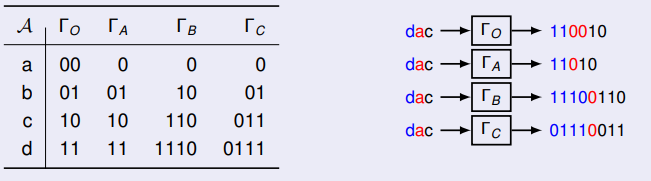
\includegraphics[scale=0.8]{12025-06-02.png}
     \end{center}
     
 
 \end{parag}
\begin{parag}{Decodability}
    We want to avoir the following problem (encoding map $\Gamma_A$ )
    \begin{align*}
        cbaad \to 100010011 \begin{cases} \to cbaad \\ \to cacad
    \end{align*}

    \begin{definition}
        The code is uniquely decodable if every concatenation of codewords has a unique parsing into a sequence of codewords.
    \end{definition}
    
    Recall that the encoding function $\Gamma$ is one to one by assumption
    \begin{subparag}{Example}
        Code $C$ or $B$ are uniquely decodable : 
        (A mettre une image 106)
    \end{subparag}
\end{parag}
 
\begin{parag}{Prefix Free codes}
    \begin{definition}
        If no codeword is a prefix of another codeword, the code is said to be prefix free.
    \end{definition}
   \begin{subparag}{Example}
        The codeword \important{01} is a prefix of \important{01}1. \\

       
   \end{subparag}
   \begin{itemize}
       \item A prefix free code is always uniquely decodable
       \item A uniquely decodable code is \important{not necessarily} prefix free
   \end{itemize}
   \begin{subparag}{A prefix code }
       A prefix free code is also called instantaneous code : 
       \begin{itemize}
           \item Think of phone numbers
           \item Think about streaming: instantaneous codes minimize the decoding delay (for given codeword length)
       \end{itemize}
   \end{subparag}
\end{parag}
 
\begin{parag}{Code for one random variable}
    We start by considering codes that encode \important{one single random variable} $ S \in \mathcal{A}$.
    \\
    To encode a sequence $S_1, S_2, \dots $ of random variables, we encode one random variable at a time.
\end{parag}

\begin{parag}{Complete tree of a code}
    Slide 113 screen.
\end{parag}
\begin{parag}{Binary tree}
    \begin{itemize}
        \item There is a \improtant{root} (the beginning)
        \item A vertex (another node)
        \item A \important{leaf} is the last vertex
        \item Which is like a (arbre généalogique)
    \end{itemize}
\end{parag}
\begin{parag}{Ternary Tree}
    The same as a binary tree but with three children.
\end{parag}

\begin{parag}{With/Without prefix}
slide 115.
\end{parag}

\begin{parag}{Decoding tree}
    \begin{itemize}
        \item Obtained from the complete tree by keeping only branches that form a codeword
        \item Useful to visualize the decoding process
    \end{itemize}
    Slide 116
\end{parag}

\subsection{Codeword length}
    \begin{itemize}
        \item The codeword length is defined the obvious way:
        \item Example: 
            \begin{center}
            \begin{tabular}{|c|c|c|}
            \hline
                $ \mathcal{A}$ & $ \Gamma_B$ & codeword lengths \\
            \hline
            \hline
                $a$ & $0$ & $1$ \\
            \hline
                $b$ & $10$ & $2$ \\ 
            \hline
                $c$ & 110 & 3 \\
            \hline
                $d$ & 1110 & 4
            \hline
             \end{tabular}
            \end{center}
         \item We would like the average codeword length to be as small as possible.
    \end{itemize}
\subsection{Kraft McMillan}
\begin{parag}{Part 1. Necessary condition for the code to be uniquely decodable}
    \begin{theoreme}
        If a $D$-ary code is uniquely decodable then its codeword length $i_1, \dots, i_M$ satisfy
        \begin{align*}
            D^{-l_1} + \cdots  + D^{-l_M} \leq i 
        \end{align*}
        Kraft's inequality
    \end{theoreme}
  \begin{subparag}{Example}
        For code $O$ we have : 
        \begin{align*}
            2^{-2} + 2^{-2} + 2^{-2} + 2^{-2} = 1
        \end{align*}
        
  \end{subparag}

\end{parag}

\begin{parag}{contrapositive of Kraft McMillan part 1}
\begin{subparag}{Example A}
    For code $A$ we have $2^{-1} + 2^{-2} + 2^{-2} + 2^{-2} = 1.25 > 1$
    .
    \\
    KRaft-McMillan's inequality is not fulfilled. \\
    There exists no uniquely decodable code with those codeword lengths.
\end{subparag}    
\end{parag}

\begin{parag}{Proof of K-MM Part I}
    We prove a slightly weaker result, namely that the codeword lengths of prefix free codes satisfy K-MM inequality.
    \\
    Let $L = \text{max}_i l_i$ be the complete tree's depth. 
    \begin{itemize}
    \item There are $D^L$ terminal leaves
        \item There are $D^{L-l_i}$
        \item No two codewords share a terminal leaf (The code is prefix free)
        \item Hence $D^{L-l_i} + D^{L-l_2} + \cdots  + D^{L-l_m} \leq D^L$
    \end{itemize}
    After dividing both sides by $D^L$ we obtain Kraft's inequality:
    \begin{align*}
        D^{-l_1} +  D^{-l_2} + \cdots  + D^{-l_M} \leq 1
   \end{align*}
    \begin{subparag}{Exercice}
        What is the \important{converse} of Kraft McMillan part 1?
        \\
        The \important{Converse} of Kraft McMillan part 1 is not true (Consider e.g. two codewords: 01 and 0101)
        \\
        However, the following statement is almost as good : 
        \begin{theoreme}
            If the positive integer $I_1, \dots, I_M$ satisfy Kraft's inequality for some positive integer $D$,then there exists a D-ary \important{prefix free code} (hence uniquely decodable) that has codewords
        \end{theoreme}
        
        This says that if the inequality is true, then we \important{can} find D \text{ such that } there exists a binary prefix which makes it decodable \important{and} prefix free!
    \end{subparag}
\end{parag}

\subsection{Important Consequence of Kraft McMillan}
\begin{parag}{Part I}
\begin{theoreme}
    If a \important{D-ary code is uniquely decodable}, then its codeword length $I_1, \dots I_M$ satisfy Kraft's inequality : 
    \begin{align*}
        D^{-l_1} + \cdots  + D^{-l_M} \leq 1
    \end{align*}
    
\end{theoreme}

\end{parag}
\begin{parag}{Part II}
    \begin{theoreme}
        If the positive integer $l_1, \dots, l_M$ satisfy Kraft's inequality for some positive integer $D$, then there exists a D-ary \important{prefix free code} that has those codeword lengths.
    \end{theoreme}
   The Kraft McMillan theorem implies that any uniquely decodable code can be substituted by a prefix free code of the same codeword lengths. 

\end{parag}

\begin{parag}{Prefix free codes}
    Our focus will be on prefix free codes. Reasons:
    \begin{itemize}
        \item No loss of optimality: codewords can be as short as for any uniquely decodable code;
        \item a prefix free codeword is recognized as soon as its last digit is seen:
            \begin{itemize}
                \item important, e.g. a phone number;
                \item advantageous to limit the decoding delay in, say streaming
            \end{itemize}
    \end{itemize}
\end{parag}

\begin{parag}{Average Codeword length}
    \begin{itemize}
        \item The typical use of a code is to encode a sequence of random variables
            \item
    \end{itemize}
    \begin{subparag}{Example}
        \begin{align*}
            \mathcal{A} = \{a, b, c, d\} \; \; D = 2
        \end{align*}
        Blackboard with table
        \begin{tabular}{cccc}
            $s \in \mathcal{A} $ & $ \Gamma (s)$ & $l(s)$ & $p(s)$ \\
            \hline \\ \hline
            \\
            $a$ & $ 0$ & 1 & 0.05 \\
            \hline 
            b & 10 & 2 & 0.05 \\
            c & 110 & 3 & 0.1 \\
            d & 1111 & 4 & 0.8
        \end{tabular}

        \begin{align*}
            \mathcal{E} [ \text{length} ] = 0.05 + 1 + 0.05 \cdot 2
        \end{align*}
        
             
        

    \end{subparag}
    \begin{definition}
        Let $l( \Gamma (s))$ be the length of the codeword assiociated to $s \in \mathcal{A}$ The average codeword length is:
        \begin{align*}
            L(S, R) = \sum_i p_s(s) i ( \Gamma (s)) 
        \end{align*}
        
    \end{definition}
    
        \begin{subparag}{Units}
            The unit of $L(S, \Gamma ) $ are \important{code symbols}
            \\
            When $D = 2$, the unit of $L(S, \Gamma )$ are bits.
        \end{subparag}
\end{parag}


\begin{parag}{Average codeword length: Lower Bound}
    \begin{theoreme}
        Let $ \Gamma : \mathcal{A} \to \mathcal{C}$ be the encoding map of a D-ary code for the random variable $S \in \mathcal{A}$ .\\
        If the code is uniquely decodable, then the average codeword length is lower bounded by the entropy of $S$ namely:
        \begin{align*} 
            H_D\left(S\right) \leq L\left(S, \Gamma\right)
        \end{align*}
        With equality if and only if for all $s \in \mathcal{A}$, $p_S\left(S\right) = D^{-l\left(\Gamma\left(s\right)\right)}$. An equivalent condition is:
        \begin{align*} 
            l\left(\Gamma\left(s\right)\right) =  \log_D \frac{1}{P_S\left(S\right)}
        \end{align*}
    \end{theoreme}
    \begin{subparag}{Proof}
        We want to prove that:
        \begin{align*}
            H(s) - \sum_s p(s)l(s) \\
            &= - \sum_s p(s) \log p(s) - \sum_s p(s)l(s) \\
            &= - \sum_s p(s)\log p(s) - \sum_s p(s) \log 2^{l(s)} \\
            &= -\sum_s p(s) \log (p(s) \cdot 2^{l(s)}) \leq \dots
        \end{align*}
        Therefore:
        \begin{align*}
            &= \sum_s p(s) \log ( \frac{1}{p(s)}2^{-l(s)}) \\
            &\leq \sum_s p(s) \left( \frac{1}{p(s)}2^{-l(s)} -1 \right) \cdot C \\
            &= (\sum_s 2^{-l(s)} - \sum_s p(s)) \cdot C \\
            &\leq 0
        \end{align*}
        
        We know that the left side is less or equal to $1$ because of the Kraft Inequality, therefore it is bounded.
        
    \end{subparag}
\end{parag}




\lecture{4}{2025-02-26}{Continue}{}


\begin{parag}{Key observation}
    The right hand side of:
    \begin{align*}
        L(S, \Gamma) = \sum_{s \in \mathcal{A}} p(s) l ( \Gamma (s))
    \end{align*}
    \begin{align*}
        H_D(S) = \sum_{s \in \mathcal{A}} p(s) \log_D \frac{1}{p_S(s)}
    \end{align*}
    are identical if $l( \Gamma (s))$
    \begin{itemize}
        \item Unfortunately $l( \Gamma (s)) = \log_D \frac{1}{p_S(s)}$ is often not possible (not an integer)
        \item How about choosing
    \end{itemize}
    
    \begin{theoreme}
        \begin{itemize}
            \item For every random variable $S \in \mathcal{A}$
        \end{itemize}
    \end{theoreme}
\end{parag}

\begin{parag}{Theorem}
    
    \begin{theoreme}
        The average codeword length of a D-ary Shannon-Fano code for the random variable $S$ fulfils: 
        \begin{align*}
            H_D(S) \leq L(S, \Gamma_{SF}) < H_D(S) + 1
        \end{align*}
        
    \end{theoreme}
   \begin{subparag}{Proof}
       it suffices to prove the upper bound (we have already proved the lower bound) 
       \\
       First suppose that we could use $l_i = -\log p_i$. The average length would be:
       \begin{align*}
           L(S, \Gamma) = \sum_i p_i l_i = \sum_i p_i (-\log_D p_i) = H_D(S)
       \end{align*}
       Instead we use $l_i = \left\lceil -\log p_i \right \rceil < - \log p_1 + 1 $
       
   \end{subparag} 

\end{parag}


\lecture{5}{2025-03-04}{Conditional Entropy}{}


\begin{parag}{Key Idea}
    Pack multiple symbols into " \textit{supersymbols}"
    \begin{itemize}
        \item $(S_1, S_2, S_3, \dots, S_n)$
        \item Now, apply our Main result to such supersymbols
    \end{itemize}
    \begin{theoreme}
        The average codeword-length of a uniquely decodable code $ \Gamma$ for $S$ must satisfy:
        \begin{align*}
            H_D(S_1, S_2, \dots, S_n) \leq L((S_1, S_2, \dots, S_n), \Gamma)
        \end{align*}
        And there exists a uniquely decodable code $ \Gamma_{SF}$ satisfying:
        \begin{align*}
            L((S_1, S_2, \dots, S_n), \Gamma_{SF}) < H_D(S_1, S_2, \dots, S_n) + 1
        \end{align*}
    \end{theoreme}
\end{parag}

\begin{parag}{Our Next Nugget}
    Understand

    \begin{subparag}{Example}
        Audio recording:
        \begin{itemize}
            \item We can easily anticipate the next image in a video, there
        \end{itemize}
    \end{subparag}

\end{parag}

\begin{parag}{KEy(simple) Independent}
    \begin{definition}
        The source models a seuquence $S_1, S_2, \dots, S_n$ of $n$ coin flips
        \\
        So $S_i \in \mathcal{A} = \{H, T\}$ where $H$ stands for heat, T for tails.
        \\
        $p_{S_i}(H) = p_{S_i}(T) = \frac{1}{2}$ for all $(s_1, S_2, \dots, S_n) \in \mathcal{A}^n$
    \end{definition}

    

\end{parag}

\begin{parag}{Not independent}
    \begin{definition}
        The source models a sequence $S_1, S_2, \dots, S_n$ of weather conditions.
        \\
        So $S_i \in \mathcal{A} = \{S, R\}$, where $S$ stands for sunny and $R$ for rainy\\
        The weather on the first day is uniformly distributed in $ \mathcal{A}$.
        \\
        For all other days, with probability $q = \frac{6}{7}$ the weather is as for the day before
    \end{definition}
    

\end{parag}


 \begin{parag}{Conditional Probability}
     Recall how to determine the conditional probability:
     \begin{align*}
         p_{X\mid Y}(x \mid y) = \frac{p_{X, Y}(x, y)}{p_Y(y)}
     \end{align*}
     It gives the probability of the event $X = x$, given that the event $Y = y$ has occured. \\ it is defined for all $y$ for which $p_Y(y) > 0$
     \begin{subparag}{Remark}
         There is good slide with good schema in slide 176-179
         
     \end{subparag}
 \end{parag}

 \begin{parag}{Conditional Expectation of $X$ given $Y = y$}
     \begin{align*}
         p_{X \mid Y}( \cdot \mid y)
     \end{align*}
     is the probability distribution of the alphabet of $X$, juste like $p_x( \cdot)$
     \begin{definition}
         The conditional expectation of $X$ given $Y = y$ is defined as:
         \begin{align*}
             \mathcal{E}[X \mid Y = y] = \sum_{ x \in \mathcal{X}}
         \end{align*}
         
     \end{definition}
     
     
 
 \end{parag}

 
 \begin{parag}{Conditional Entropy of $X$ given $Y = y$}
     $p_{X \mid Y}( \cdot \mid  y)$ is a probability distribution on the alphabet of $X$, juste like $p_X( \cdot)$ Every probability distribution has an entropy associated to it:
     \begin{itemize}
         \item $p_x( \cdot) \to H(X)$
         \item $p_{ X \mid  Y}( \cdot \mid y) \to H(X \mid Y = y)$
     \end{itemize}
     \begin{definition}
         The conditional entropy of $X$ given $Y = y$ is defined as:
         \begin{align*}
             H_D ( X \mid Y = y) = - \sum_{x \in \mathcal{X}} p_{X \mid Y}(
         \end{align*}
         
     \end{definition}
     \begin{subparag}{Example}
         A faire
         
     \end{subparag}
 
 \end{parag}
 \begin{parag}{Entropy Bounds}

     \begin{theoreme}
         The conditional entropy of a discrete random variable $X\in \mathcal{X}$ conditioned on $Y = y$ satisfies:
         \begin{align*}
             0 \leq H_D(X \mid Y = y) \leq \log_D \mid \mathcal{X} \mid
         \end{align*}
     With equality on the left iff $p_{X \mid Y}(x, y) = 1$ for some $x$, and with equality on the right iff $p_{X \mid Y}(x \mid y) = \frac{1}{\mid \mathcal{X}\mid }$
         
     \end{theoreme}
     The proff is identical to our proof of the basic entropy bounds
 
 \end{parag}
 
 \begin{parag}{Example}
     Question?
     \\
     Do we also have the following entropy bound:
     \begin{align*}
         H_D(X \mid > = y) \overbrace{ \leq}^{???} H_D(X)?
     \end{align*}
     Answer: no.

     \begin{subparag}{Example}
         (Or " \textit{counterexample}" if better), Juste for ease of calculation, let us set $ \delta = 0$ (but this is not necessary for the example to work). Then, we have:
         \begin{align*}
             H_D(X \mid Y = 0) h_D( \epsilon) \text{ and } H_D(X \mid Y= 1) = 0
         \end{align*}
         where $h_d( \cdot)$ is the binary entropy function (with $\log_D( \cdot)$). But we have:
         \begin{align*}
             H_D(X) = h_D( \frac{1 - \epsilon}{2})
         \end{align*}
     \end{subparag}
     \begin{framedremark}
         Conditional entropy can either go up or down (if we give the answer the entropy is $0$)
     \end{framedremark}
 \end{parag}
 \begin{parag}{Conditional Entropy of $X$ given $Y$}
     The most useful and impactful definition is the \textit{average} conditional entropy of $X$ given $Y = y$, averaged over all values of $y$ under the marginal distribution $p_Y(y)$. Formally, we thus define:
    \begin{definition}
    The conditional entropy $X$ given $Y$ is defined as:
    \begin{align*}
        H_D(X \mid Y) = \sum_{y \in \mathcal{Y}}p_Y(y) \left( - \sum_{x \in \mathcal{X}} p_{X \mid Y}(x \mid y)\log_D p_{X \mid Y} (x \mid y) \right)
    \end{align*}
\end{definition}

\begin{subparag}{Example}
    For the Bit flipper channel, we have;
    \begin{align*}
        H_D( X \mid  Y) = p(Y = 0) H_D(X \mid  Y = 0) + p(Y = 1)H_D( X \mid Y = 1)
    \end{align*}
    We search now:
    \begin{align*}
        H(X \mid  Y) = p(Y \text{ is Head}) H(X Y \text{ is head}) + p( Y \text{ is Tail}) H(X \mid  Y \text{ is tail}) = \frac{1}{2} \cdot 1 + \frac{1}{2} \cdot 0 = \frac{1}{2}
    \end{align*}
\end{subparag}
\end{parag}

\begin{parag}{Conditional Entropy of $X$ given $Y$}
    \begin{theoreme}
        The conditional entropy of discrete random variable $X \in \mathcal{X}$ conditioned on $Y$ satisfies:
        \begin{align*}
            o \leq H_D(X \mid  Y) \leq \log_D \mid \mathcal{X} \mid
        \end{align*}
        With equality on the left iff for every $y$ there exists and $y$ \text{ such that } $p_{X \mid  Y}( x \mid  y) = 1$ and with equality on the right iff $p_{X \mid  Y}(x \mid  y) = \frac{1}{ \mid \mathcal{X} \mid}$ for all $x$ and all $y$.
    \end{theoreme}
    This follows directly from our bounds on $H_D(X \mid Y = y)$
    \begin{framedremark}
        Having $p_{X \mid  Y}$
    \end{framedremark}
    We know that $p(X \mid Y) = \frac{1}{ \mid \mathcal{X} \mid}$  for all $y$.
    \\
    \begin{align*}
        p(x) &= \sum_{y \in \mathcal{Y}}p(y) p(x \mid  y) \\
        &= \sum_y p(y) \frac{1}{ \mid \mathcal{X} \mid} \\
        &= \frac{1}{ \mid \mathcal{X} \mid} \cdot \sum_y \overbrace{p(y)}^{=1}
    \end{align*}
    
    
    

\end{parag}





 \begin{parag}{Conditioning Reduces Entropy}
     The following bound is important and impactful (and also intuitively pleasing!)
     \begin{theoreme}
         For any two discrete random variables $X$ and $Y$,
         \begin{align*}
             H_D(X \mid Y) \leq H_D(X)
         \end{align*}
         with equality iff $X$ and $Y$ are independent random variables
     \end{theoreme}
     In words, \important{On average}, the uncertainty about $X$ can only become smaller if we know $Y$.
     \begin{framedremark}
         As we have seen, this is not true point-wise: We may have $H_D( X \mid  Y = y) > H_D(X)$ for some values of $y$.
         \\
         It works only on average.
     \end{framedremark}
     \begin{subparag}{Proof}
         \begin{align*}
             H(X \mid  Y) - H(X) &=\\
                                 &= \sum_yp(y) \left( -\sum_xp(x \mid  y) \log p(x \mid  y) \right) + \sum_x p(x) \log p(x)\\
                                 &= \sum_{x, y}p(y)p(x \mid y) \log \frac{1}{p(x \mid y)} + \sum_{x, y} p(y \mid x)p(x) \log p(x)\\
                                 &= \sum_{x, y}p(x, y) \log \frac{p(x)}{p(x \mid y)} \\
                                 &\leq \sum_{x, y}p(x, y) \left( \frac{p(x)}{p(x \mid  y}- 1 \right) \cdot \log e
                                 &= \sum_{x, y}p(x, y) \left \frac{p(x)p(y)}{p(x, y)} -1 \right) \cdot \log(e) \\
                                 &= \sum_{x, y} \left( p(x)p(y) - p(x, y) \right) \log(e)\\
                                 &= \left( \left( \sum_{y}p(x)p(y) \right) - \left(\sum_x p(x)p(y) \right) \right)
         \end{align*}
         
     \end{subparag}
     
 
 \end{parag}
 
 
 \begin{parag}{Conditional Entropy of $f(x)$}
     Let $X$ be an arbitrary random variable. Let $f(x)$ be a (deterministic) function of $x$.\\
     \begin{align*}
         H(f(x) \mid X) = 0
     \end{align*}
\begin{subparag}{Proof}
    To find this conditional entropy:
    \\
    Let $Y = f(x)$
    \begin{align*}
       p(y \mid  y) = \begin{cases}
           1, \; \; \; y = f(x) \\ 0, \; \; \; y \neq f(x)
       \end{cases} 
    \end{align*}
       the probability that $y$ is $f(x)$ is only true if $f(x) = y$.
       \\
       This implies that the entropy is equal to $0$:
       \begin{align*}
           H(y \mid  x) = 0
       \end{align*}
       
\end{subparag}
     
 
 \end{parag}

 \begin{parag}{Conditioning reduced Entropy}
     A generalization of the previous bound is also interest to us:
     \begin{theoreme}
         For any three discrete random variables $X, Y$ and $Z$, 
         \begin{align*}
             H_D(X \mid  Y, Z) \leq H_D(X \mid  Z)
         \end{align*}
         With equality iff $X$ and $Y$ are conditionally independent random variables given $Z$ (that is, if and only if $p(x, y \mid z) = p(x \mid z)p( y \mid z)$ for all $x, y, z$,
     \end{theoreme}
     You can see it as make the $Z$ fall which makes it $p(x, y) = p(x)p(y)$
     \begin{subparag}{Proof}
         It is only mathematics:
        \begin{align*}
            H_D(X \mid  Y, Z) - H_D(X \mid  Z) &= \mathbb{E} \left[ \log_D \frac{1}{p_{X \mid  Y, Z}(X \mid Y, Z)} \right] + \mathbb{E}[\log_D p_{X \mid Z}(X \mid Z)] \\
                                            &= \mathbb{E}\left[\log_D \frac{p_{X \mid Z}(X \mid Z)}{p_{X \mid  Y}(X \mid Y, Z)} \right]\\ 
                                            &= \mathbb{E}\left[ \log_D \frac{p_{X \mid Z}(X \mid  Z) p_{Y \mid  Z}(Y \mid Z) p_Z(Z)}{nique sa mere} \right
     \end{align*}
      
     \end{subparag}
 \end{parag}
 
 















\lecture{6}{2025-03-04}{Conditional Entropy review}{}
\begin{parag}{Main definitions}
    We have here two mains definitions:
    \\
    The entropy for for a "\textit{case}" of a random variable:
    \begin{align*}
        H(X \mid  Y = y) = - \sum_x p(X \mid  y) \log p(X \mid y)
    \end{align*}
    And, the conditional entropy on a random variable:
    \begin{align*}
        H(X \mid  Y) &= \sum_y p(y) H(X \mid  Y = y) \\
                     &= - \sum_y \sum_x p(x, y) \log p(x \mid  y)
    \end{align*}
    The main thing to understand here is that $H(X \mid  Y)$ is the \textit{Generalization} of the first definition. It is all the possible values of $Y$ together. This is why we sum up all possible value of $y$. The second way to write $H(X \mid  Y)$ is like taking all the possible pairs together and calculating the entropy of each pairs.
    \\
    \textbf{Main Result}: The main result behind this is:
    \begin{align*}
        0 &\leq H(X \mid  Y = y) \leq \log \mid \mathcal{X} \mid \\
        0 &\leq H(X \mid Y) \leq \log \mid  \mathcal{X} \mid \\
    \end{align*}
    And the inequality:
    \begin{formule}
        \begin{align*}
            H(X \mid  Y) \leq H(X)
        \end{align*}
    \end{formule}
   \begin{subparag}{Conditional entropy of $f(x)$}
       Let $X$ be an arbitrary random variable.
       \\
       Let $f(x)$ be a (deterministic) function of $x$:
       \begin{align*}
           H(f(x) \mid  x) = 0
       \end{align*}
       For example:
       \begin{align*}
           X \in \{0, 1, 2, 3\} \\
           f(x) = X \mod 2
       \end{align*}
       
       Which is:
       \begin{align*}
           f(x) = \begin{cases}
               0 \text{ if x is even} \\
               1 \text{ if x is odd}
           \end{cases}
       \end{align*}
      Then,
      \begin{align*}
          P(f(x) \mid X) = \begin{cases}
              0, \text{ if } x = 0, 2 \\
              1, \text{ if } x = 1, 3
          \end{cases}
      \end{align*}
      If we now compute the entropy for $X = 0$ and $X = 1$ etc...,  we get:
      \begin{align*}
          H(f(x) \mid  X = 0) = 0 \\
         H(f(x) \mid  X = 1) = 0 \\
         \vdots
      \end{align*}
   \end{subparag} 
\end{parag}

\begin{parag}{Lisa rolls two dice}
    Lisa rolls two dice and annoucnes the sum $L$ written as a two digit number.
    \\
    The alphabet of $L = L_1L_2 = \{02, 03, 04, 05, 06, 07, 08, 09, 10, 11, 12\}$ Where the alphabet of $L_1 = \{0, 1\}$ and the alphabet of $L_2 = \{0, 1, 2, \dots, 9\}$.
    \\
    We are looking for the probability that $L_2 = 2$ knowing that $L_1 = 1$:
    \begin{align*}
        p_{L_2 \mid  L_2}(2 \mid  1)
    \end{align*}
    What we are doing here is the joint distribution:
    \begin{align*}
        p_{L_2 \mid  L_1}(2 \mid  1) = \frac{P_{L_1, L_2}(1, 2)}{P_{L_1}(1)} = \frac{ \frac{1}{36}}{ \frac{1}{6}} = \frac{1}{6}
    \end{align*}
    After running over all possible values for $(i, j)$, we obtain:
    \begin{center}
    \begin{tabular}{|c|c|c||c|}
        $L_2 = j$ $L_1 =i$ & 0 & 1 & $p_{L_2}(j)$ \\
        \hline 
        \hline
        0 & 0 & $\frac{3}{36}$ & $ \frac{3}{36}$ \\
        1 & 0 & $ \frac{2}{36}$& $ \frac{2}{36}$ \\
        2 & $ \frac{1}{36}$ & $ \frac{1}{36}$ & $ \frac{2}{36}$ \\
        $ \vdots$ &$ \vdots$ &$ \vdots$ &$ \vdots$ \\
        $p_{L_i}(i)$ & $ \frac{5}{6}$ & $ \frac{1}{6}$ & 
        \hline
    \end{tabular}
    \end{center}
    
   now you can do the same with conditional probability and then after computing all those value:
   \begin{align*}
       H(L_2 \mid  L_1) = \frac{5}{6} \cdot 2.857 + \frac{1}{6} \cdot 1.459 = 2.624 \text{ bits}
   \end{align*}
   Now we can observe that:
   \begin{align*}
       2.624 = H(L_2 \mid  L_1) \leq H(L_2) = 3.22
   \end{align*}
   Which says that on average, knowing something takes out some randomness
   
   
\end{parag}

\begin{parag}{The chain rule for entropy}
    Recall that the joint entropy of two random variables $X, Y$ is completely naturally defined as:
    \begin{align*}
        H_D(X, Y) = - \sum_x \sum_y p_{X, Y}(x, y) \log_Dp_{X, Y}(x, y)
    \end{align*}
    Or as seen earlier:
    \begin{align*}
        H_D(X, Y) = H_D(X) + H_D(Y)
    \end{align*}
    
    Using the fact the $p_{X, Y}(x, y) = p_X(x)p_{Y \mid  X} ( y \mid  x)$, we can write this as:
    \begin{align*}
        H_D(X, Y) &= - \sum_x p_X(x) \left( \sum_Y p_{Y \mid  X}( y \mid  x) \log_D(p_X(x)p_{Y \mid  X}(y \mid  x)) \right) \\
                  &= - \sum_x p_X(x) \left( \sum_yp_{Y \mid  X}(y \mid  x) (\log_D p_X(x) + \log_Dp_{Y \mid  X}(y \mid x)) \right) \\
                  &= - \sum_x p_X(x) \left[ \left( \sum_y p_{Y \mid  X} (y \mid x) \log_D p_X(x) \right) + \left( \sum_y p_{Y \mid  X} (y \mid  x) \log_D p_{Y \mid  X}(y \mid  x) \right) \right] \\
                  &= H(X) + H(Y \mid  X)
    \end{align*}
    
    \begin{theoreme}
        \begin{align*}
            H(X, Y) = H(X) + H(Y \mid  X)
        \end{align*}
    \end{theoreme}
    \begin{subparag}{Professor remark}
        Firstly:
        \begin{align*}
            H(Y, X) = H(X, Y)
        \end{align*}
        Which is either proved by:
        \begin{align*}
            H(Y,X ) &= H(Y) + H(X \mid  Y) \\
                &= H(X, Y)
        \end{align*}
        The relation proved before in words it:
       \\
       To find the joint entropy of two random variables, we can first calculate the entropy of one of the two, and then add to it the conditional entropy of the second, given the first.
    \end{subparag}
\end{parag}

\begin{parag}{The chain rule entropy}

    \begin{theoreme}
        Let $S_1, \dots, S_n$ be discrete random variables. Then:
        \begin{align*}
            H_D(S_1, S_2, \dots, S_n) = H_D(S_1) + H_D(S_2 \mid S_1) + \cdots + H_D(S_n \mid S_1, \dots, S_{n-1})
        \end{align*}
    \end{theoreme}

    The above result says that the uncertainty of a collection of random variables (in any order) is the uncertainty of the first, plus the uncertainty of the second when the first is known, plus the uncertainty of the third when the first two are know, etc$ \dots$
    \\
    Let us see how:
    \begin{align*}
       &H(\underbrace{S_1, S_2, \dots, S_{n-1}}_{=  Z}, S_n) \\
        &= H(Z) + H(S_n \mid Z)  \\
        &= H( \underbrace{S_1, S_2, \dots, S_{n-2}}_{= Z'}, S_{n-1}) + H(S_n \mid S_1 \dots, S_{n-1}) \\
        &= H(Z') + H(S_{n-1} \mid Z') + H(S_n \mid S_1, \dotsS_{n-1}
    \end{align*}
    Until we get $Z^{' \cdots'} = S_1$.
    
    \begin{subparag}{Example}
        Let $X, Y, Z$ be discrete random variables. We have:
        \begin{align*}
            H(X, Y, Z) &= H(X) + H(Y \mid X) + H(Z \mid  X, Y) \\
&= H(X) + H(Z \mid X) + H(Y \mid  X, Z) \\
&= H(Y) + H(X \mid Y) + H(Z \mid  X, Y) \\
&= H(Y) + H(Z \mid Y) + H(X \mid  Y, Z) \\
&= H(Z) + H(X \mid Z) + H(Y \mid  X, Z) \\
&= H(Z) + H(Y \mid Z) + H(X \mid  Y, Z) 
        \end{align*}
        
        
    \end{subparag}
    \begin{theoreme}
        Let $S_1, \dots, S_n$ be discrete random variables. Then:
        \begin{align*}
            H(S_1, S_2, \dots, S_n) \leq H(S_1) + H(S_2) + \cdots  + H(S_n)
        \end{align*}
        With equality iff, $S_1, \dots, S_n$ are independent
    \end{theoreme}
   \begin{subparag}{Proof}
        \begin{align*}
       H(S_1, S_2, S_3) &= H(S_1) + H(S_2 \mid  S_1) + H(S_3 \mid  S_1, S_2) \\
                         &\leq H(S_1) + H(S_2) + H(S_3)
   \end{align*}
   \end{subparag}
\end{parag}
\begin{parag}{Another way around}
    Sometimes it is convenient to compute the conditional entropy using the chain rule for entropies. For instance:
    \begin{formule}
        \begin{align*}
            H(X \mid  Y) = H(X, Y) - H(Y)
        \end{align*}
    \end{formule}
    It can be useful to make it easier to compute $H( X \mid  Y)$ because on the right side, it is only marginal entropies with $p \log p$ which are  \textit{"easy to compute}"
    \\
    \begin{corollaire}
        \begin{align*}
            H(X, Y) \geq H(X) \\
            H(X, Y) \geq H(Y)
        \end{align*}
    \end{corollaire}
    The above inequalities follow from the chain rule for entropies and the fact that entropy (condition or not) is nonnegative.
    
\end{parag}

\begin{parag}{Example}
    From lisa rolls two dice:
    \begin{align*}
        H(L_1, L_2) &= 3.2744 \\
        H(L_1) &= 0.6500 \\
        H(L_2) &= 3.2188
    \end{align*}
    We compute:
    \begin{align*}
        H(L_2 \mid  L_1) &= H(L_1, L_2) - H(L_1) = 3.2744 - 0.6500 = 2.6254 \\
        H(L_1 \mid  L_2) &= H(L_1, L_2) _ H(L_2) = 3.2744 - 3.2188 = 0.056
    \end{align*}
    And verify that indeed:
    \begin{align*}
        H(L_1 \mid  L_2) \leq H(L-1) \leq H(L_1, L_2) \\
        H(L_2 \mid  L_1) \leq H(L_2) \leq H(L_1, L_2)
    \end{align*}
    
    
    

\end{parag}


\subsection{Random Processes}
\begin{parag}{A.K.A Source models}
    \begin{definition}
        The source models a sequence $S_1, S_2, \dots, S_n$ of $n$ coin flips\\
        So $S_i \in \mathcal{A} = \{H, T\}$, where $H$ stands for heads, $T$ for tails, $i = 1, 2, \dots, n$ \\
        $p_{S_i}(H) = p_{S_i}(T) = \frac{1}{2}$ for all $i$, and coin flips are independent.\\
     Hence,
     \begin{align*}
         p_{S_1, S_2, \dots, S_n}(S_1, S_2, \dots, S_n) = \frac{1}{2^n}, \; \; \forall (S_1, S_2, \dots, S_n) \in \mathcal{A}^n
     \end{align*}
     
    \end{definition}
\begin{definition}
    The source models a sequence $S_1, S_2, \dots, S_n$ of weather conditions.
    \\
    So $S_i \in \mathcal{A} = \{S, R\}$, where $S$ stands for sunny and $R$ for rainy, $i = 1, 2, \dots, n$. \\
    The weather on the first day is uniformly distributed in $ \mathcal{A}$. \\
    For all other days, with probability $q = \frac{6}{7}$ the weather is as for the day before
\end{definition}
What we can see here that is the conditional probability, for example:
\begin{align*}
    p(S_2 = \text{ sun} \mid S_1 = \text{ sun}) = q \\
    p(S_2 = \text{ rain} \mid  S_1 = \text{ sun}) = 1 - q
\end{align*} 
However:
\begin{align*}
   p(S_3 = \text{sun} \mid S_1 = \text{sun}, S_2 = \text{sun})\\
   = p(S_3 = \text{ sun} \mid S_2 = \text{ sun}) = q
\end{align*}
More generally:
\begin{align*}
    P(S_n \mid  S_1, S_2, \dots, S_{n-1}) = p(S_n \mid  S_{n-1})
\end{align*}


    

\end{parag}



\lecture{7}{2025-03-11}{Entropy and algorithm}{}
\begin{parag}{Experience little play}
    \begin{itemize}
        \item Think of something
        \item Ask yes or no question
        \item Find the answer
    \end{itemize}
    the game was called twenty questions in old U.S tv. We want to use entropy to understand this game.
\end{parag}
\begin{parag}{Last Week}
\begin{align*}
    H_D(X) = H_D(P) - -\sum_x p(x) \log_D p(x)
\end{align*}

We also saw those two bounds:
\begin{align*}
    0 \leq H_D(X) \leq \log_D \mid  \mathcal{A} \mid
\end{align*}
Information is always about option, more options you have, more information (the first way to introduce \textit{"entropy"})\\
We also saw:
\begin{align*}
    H(X \mid  Y = y) = - \sum_x p(x \mid  y) \log_Dp(x \mid  y)\\
    H(X \mid  Y = y) = - \sum_y \dots
\end{align*}
And we also saw that on average:
\begin{align*}
    H(X \mid  Y) \leq H(X) \\
    H(X \mid  Y, Z) \leq H(X \mid  Y) \leq H(X)
\end{align*}

We also saw the chain rule:
    \begin{align*}
       H(S_1, S_2, S_3, S_4) \\
       = H(S_2, S_4, S_1, S_3)
    \end{align*}
    The order in entropy doesn't matter,
    \begin{align*}
        = H(S_1) + H(S_2 \mid  S_1) + H(S_3 \mid  S_1, S_2) + H(S_4 \mid  S_1, S_2, S_3)
    \end{align*}
    An intresting way to use this, is if we combine the inequalities and the chain rule. The equality on the right sight is true if and only if $X$ and $Y$ are independent. there fore:
    \begin{align*}
        H(S_1, S_2, S_3, S_4) = H(S_1) + H(S_2) + H(S_3) + H(S_4)
    \end{align*}
    this equality is true if and only if $S_1, S_2, S_3, S_4$ are independent.
    
\end{parag}


\begin{parag}{The 20 question problem}
    Let $X$ be a random variable. What is the minimum number of "yes/no" question needed to identify $X$?, which question should be asked.
\end{parag}
\begin{parag}{Solution}
    Let us consider a binary code $ \Gamma$ for $X \in \mathcal{X}$
    \\
    Once $ \Gamma$ is fixed, we know $x \in \mathcal{X}$ if and only if we know the codeword $ \Gamma(x)$. The strategy consists in asking the $i$th question so as to obtein the $i$th bit of the codword $ \Gamma(x)$.
    \\
    The expected number of question $L(X, \Gamma)$, which is minimized if $ \Gamma$ is the encoding map of Huffman code

    \begin{subparag}{Example}
        Suppose that we know that $ \mathcal{X} = \{ $ cat, dog, pony$\}$, with:
        \begin{align*}
            p(cat) = \frac{1}{2}\\
            p(dog) = \frac{1}{4} \\
            p(pony) = \frac{1}{4}
        \end{align*}
        We want to make it the best way, the question we should ask is:
        \begin{itemize}
            \item is the animal a cat?

        \end{itemize}
       
        \begin{center}
            \begin{tabular}{cccccc}
                $X$ & a & b & c & d & e 
           \hline

        \end{tabular}
        \end{center}
        
        
    \end{subparag}
    We then do a Huffman tree:
    \begin{center}
        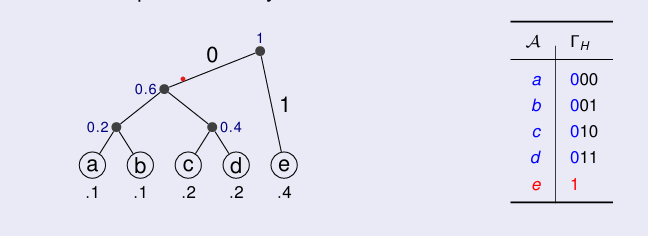
\includegraphics[0.7]{12025-03-11.png}
    \end{center}
    We know here that this, will be optimal
\end{parag}
\begin{parag}{Optimality}
    We have seen that a prefix free code for $X \in \mathcal{X}$ leads to a querying strategy to find the realization of $X$.
    \\
    Similarly, a deterministic querying strategy leads to a binary prefix-free code for $X$. Here is why:
    \begin{itemize}
        \item Before the first question we know that $x \in \mathcal{X}$
        \item Without loss of generality, the first question can be formulated in terms of "is $x \in \mathcal{A}$"? for some $ \mathcal{A} \subset \mathcal{X}$, (The choice of $ \mathcal{A}$ is determined from the strategy, that we fix once and for all)
        \item Is the answer is YES, the we know that $x \in \mathcal{A} \subset \mathcal{X}$. Otherwise $x \in A^c \subset \mathcal{X}$. Either way we have reduced the size of the set that contains $x$.
        \item We continue asking similar questions until the value of $x$ is fully determined, the we stop.
    \end{itemize}
    Here, the sequence of Yes or no answers is a binary codeword associated to $x$. The code obtained when we consider all possible values of $x$ is a binary prefix-free code. Since the tree is prefix free, its averag codeword-length cannot be smaller than that of a Huffman code.
\end{parag}

\begin{parag}{Sorting via pairwise comparisons}
    Given an \important{unsorted} List with $n$ elements.
    \\
    For example $l = [c, a, b]$ with $n = 3$
    \\
    \textbf{Repeat:}
    \begin{enumerate}
       \item Select two position $1 \leq i \leq j \leq n$
       \item Compare and swap:
           \begin{itemize}
               \item If $x_i > x_j$
               \item Then swap elements $ x_i \iff x_j$
               \item Else do nothing
           \end{itemize}
    \end{enumerate}
    One way to understands how it works:
\begin{center}
    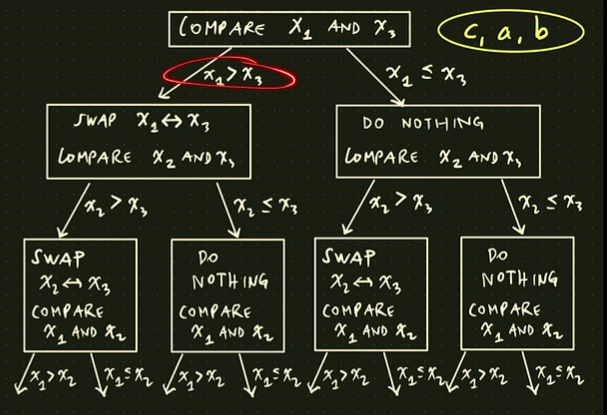
\includegraphics[scale=0.7]{22025-03-11.png}
\end{center}
The first observation:\\
The sequence of pairwise comparisons must identify the exact order of the unsorted list.
\\
The second observation:\\
The sequence of pairwise comparisons in a uniquely decodable (actually, prefix-free) binary code for $x$.\\
There fore, we must have:
\begin{align*}
    \mathbb{E}[ \text{number of comparisons}] \geq H_2(X)
\end{align*}
However what is the $X$? We see it as a random variable because we don't really know what the unsorted list is.\\
For example $n = 3$ we have $ \mathcal{X} = \{ abc, acb, bac, bca, cab, cba\}$ where $ \mathcal{X}$ is the set of all permutations.
\\
However what is $p(x)$? Here, we want to talk  about our algorithm working for all $p(x)$.
\\
\begin{align*}
    E &\geq max_{p(x)}H_2(X) = \log_2 \mid \mathcal{X} \mid \\
    &= \log_2 n!
\end{align*}
We already know a bounds on factorial:
\begin{align*}
    \frac{n^n}{e^{n-1}} \leq n! \leq \frac{n^{n+1}}{e^{n-1}}
\end{align*}

Therefore:
\begin{align*}
    H_2(x) &\approx \log_2 \frac{n^n}{e^{n-1}} \\
           &= n \log_2n - (n-1)\log_2 e
\end{align*}
Which is \textit{"dominated"} by $n\log_2 n$

\end{parag}

\begin{parag}{Billard Balls}
    There are 14 billards balls numbered as shown:
\begin{center}
    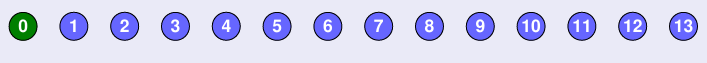
\includegraphics[scale=0.6]{32025-03-11.png}
\end{center}
Among balls $1-13$, at most one \textbf{could} be heavier/lighter than the others. What is the minimum number of weightings to simultaneously determine:
\begin{itemize}
    \item If one ball is different
    \item if there is such a ball which one, 
        \item And whether the different ball is heavier/lighter
\end{itemize}
Here we want to use entropy to solve this problem. The goal here is to associated the number of weightings to code. The goal is to see it as a tree.
\begin{center}
    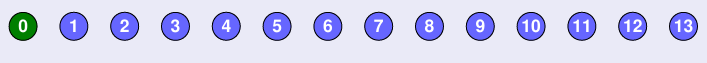
\includegraphics[scale=0.5]{32025-03-11.png}
\end{center}
The steps of picking two sets is \textit{"mandatory"} we have to pick two sets in order to compare something, and in order to compare something, you have to compare something...\\
From this comparisons, there will be three possibilities. with three possibilites, We are specifying a Ternary code. 
%\begin{framedremark}
 %   A remark during the course was:
  %  \begin{center}
    %    \textit{"Why can't we use binary, where we take the two inequalities together and the not equal alone?}
   % \end{center}
    The issue here is that we are losing information, yes we only get a binary tree however we wouldn't be able to have the same amount of information as with  a ternary tree. \\
    What we are saying here is, with any strategy to solve this problem \important{can} be written in this way. Hence we can read this tree as a ternary code.
%\end{framedremark}
\begin{subparag}{But a code for \important{What}?}
    What are we finding with this code?\\
    A code for $X$:
    \begin{itemize}
        \item $X = 0$: all balls are equals
        \item $X = +1$: ball $1$ is heavier
        \item $\vdots$ 
        \item $X = +13$ ball $13$ is heavier
        \item $X = -1$ balle $1$ is lighter
        \item $\vdots$
        \item $X = -13$ ball $13$ is lighter
    \end{itemize}
    Then we know that $ \mid \mathcal{X} \mid = 27$. This is one way to answers those question.
    \begin{enumerate}
        \item If $X = 0$ or not (then there is or not a different ball)
        \item Then  $ \mid X \mid $ gives us the information
        \item the sign of $X$ if the ball is heavier or lighter
    \end{enumerate}
    \textbf{Observation}
    The number of weighings  is equal to the length of the ternary codeword
\end{subparag}
Then:
\begin{theoreme}
    \begin{align*}
        \mathbb{E}[ \text{number of weighings}] \geq H_3(X)
    \end{align*}
\end{theoreme}
It has to be three by the way the problem is stated. The code is ternary \important{Therefore} the base for the entropy is $3$.\\
Moreover, our strategy must work \important{irrespective} of the probability distribution of $X$.
\\
We can also see:
\begin{theoreme}
    \begin{align*}
        \mathbb{E}[ \text{number of weighings}] \geq  \text{max}_{p(x)}(H_3(X))
    \end{align*}
\end{theoreme}
Where in our example gives us:
\begin{align*}
    \log_3 27 = 3
\end{align*}
\begin{framedremark}
    It doesn't need the be an integer it is only the professor that choose on purpose to make it clean
\end{framedremark}
\begin{subparag}{But does there indeed exists such a code}
    \textbf{FACT}:
    \begin{center}
        \important{Entropy} does \important{not} guarantee the existence of such a strategy
    \end{center}
   Entropy serves as a lower bound and \important{not} the best way to do it.  
\end{subparag}
    But can what if? \\
    Let us suppose it exists! Then entropy tells us a few basic facts.
\end{parag}
\begin{parag}{Fact 1}

         \important{if} $3$ weighings $S_1, S_2, S_3$ uniquely specify $X$, Then we \important{must have}:
            \begin{align*}
                H_3(X) = H_3(S_1, S_2, S_3)
            \end{align*} 
    
            \begin{subparag}{Proof}
                \begin{align*}
                    H(X, S_1, S_2, S_3) &= H(X) + \overbrace{H(S_1, S_2, S_3 \mid  X)}^{=0} \\
                                        &= H(S_1, S_2, S_3) + \overbrace{H(X \mid  S_1, S_2, S_3)}^{=0} \\
                \end{align*}
               It is true because if we know $S_1, S_2, S_3$ then we know all $X$ then the entropy of $0$. \\
               For $H(X \mid  S_1, S_2, S_3)$, because $S_1, S_2, S_3$ uniquely specify $X$ then knowing them implies that this entropy is $o$.
                
            \end{subparag}
  
\end{parag}


\begin{parag}{Fact 2}
    \important{If} 3 weighings $S_1, S_2, S_3$ uniquely specify $X$, then we must have:
    \begin{itemize}
        \item $S_1, S_2, S_3$ uniformly distributed
        \item $S_1, S_2, S_3$ independent
    \end{itemize}

    \begin{subparag}{Proof}
        \begin{align*}
            H_3(S_1, S_2, S_3) &= 3
        \end{align*}
        This is a \textit{must}.\\
        But also:
        \begin{align*}
            H_3(S_1) + H(S_2 \mid  S_1) + H(S_3 \mid S_1, S_2) \leq H_3(S_1) + H(S_2) + H(S_3) \\
            \leq \log_3 3 + \log_3 3 + \log_3 3
        \end{align*}
        Where it is an equality if and only if the distribution is uniform and independent.
        
        
    \end{subparag}
    
   
\end{parag}
\begin{parag}{Example}


Let's see how to actually find a way to ask those question:
\begin{center}
    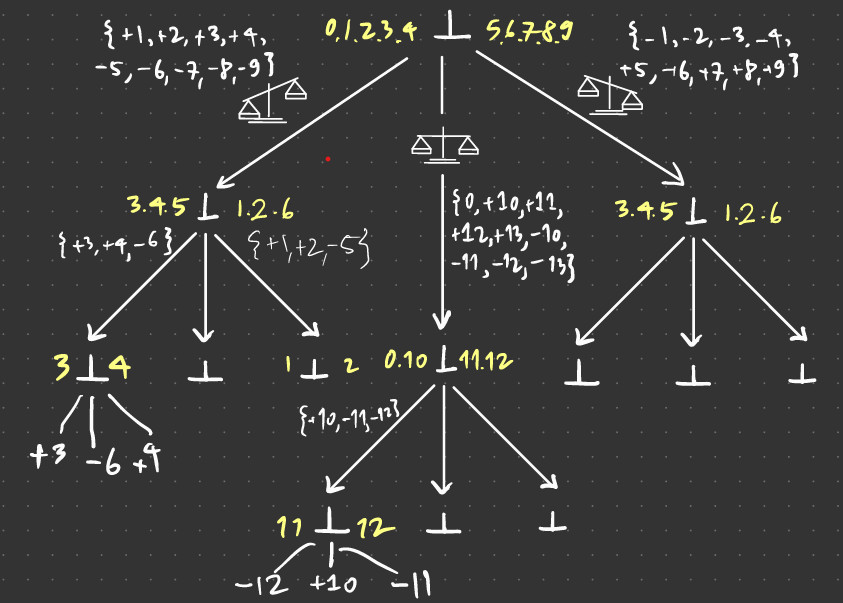
\includegraphics[scale=0.7]{52025-03-11.png}
\end{center}


\end{parag}

\lecture{8}{2025-03-12}{Prediction, learning, and Cross-Entropy-Loss}{}

\begin{parag}{Billard Balls}
    Can we use the 20 questions approach to solve the 14 bullars riddle?
    \begin{subparag}{Answer}
        No, because the kind of questions that we can "ask", when wa are weighing, is quite limited.\\
        For instance, the first question cannot be "is $1$ or $2$ heavy?".
        
    \end{subparag}

\end{parag}
\begin{parag}{Strategies}
    But is there a strategy that requires only $3$ weighings?
    \\
    From source compression, we can establish the following facts?
    \begin{itemize}
        \item For each weighings, the three outcomes must be equally likely
        \item The weighings must be independent of each other
    \end{itemize}
    \begin{framedremark}
        It is because we carefully selected the numbers (alphabet size of 27; each weighing has $3$ possible outcomes) that there is a strategy that exactly matches the entropy lower bound $3$ weighings. If you change the numbers, it will not generally be true that there is a strategy that \textit{exactly} matches the lower bound.
    \end{framedremark}
\end{parag}
\subsection{Prediction, Learning and cross-Entropy Loss}
The goal here is to change the way to use entropy, entropy has always be seen as something that \textit{means} something, a lower bound, a quantity of information. Here we will use it to do calculation juste like a \textit{tool}.
\begin{parag}{Example}
\begin{center}
    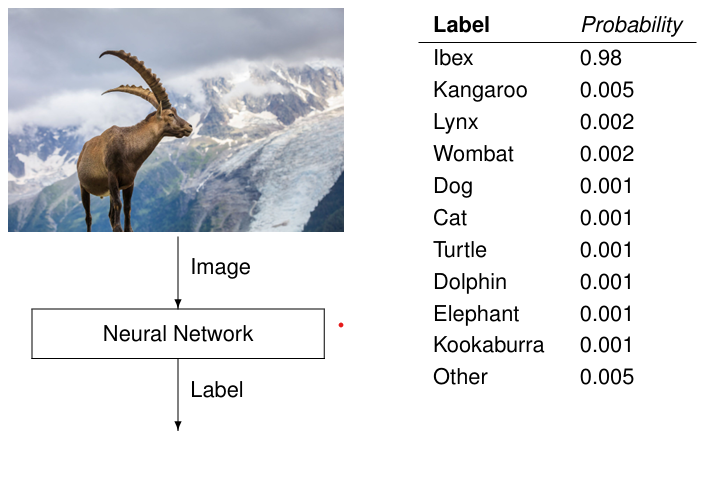
\includegraphics[scale=0.6]{12025-03-12.png}
\end{center}
\begin{framedremark}
    There weren't probability at this time in the slide so imagine without it
\end{framedremark}

The question we want to ask is, \textit{"Is our neural network performing well"}\\
\begin{itemize}
    \item Given an image $ \mathcal{X}$
    \item Our machine (Neural network)
    \item Outputs $Q(x)$
    \item The label: Label$(x)$
\end{itemize}
\begin{subparag}{Zero-one loss}
    \begin{align*}
        L\{Q(x) \neq \text{Label}(x)\}\\
        = \begin{cases}
            1 \text{ if } Q(x) \neq \text{Label}(x)\\
            0 \text{ if } Q(x) = \text{Label}(x)
        \end{cases}
    \end{align*}
    Given a lot of image, we want to have a \important{Classification error}:
    \begin{align*}
        \frac{\sum_{ \mathcal{X}} L\{Q(x) \neq \text{Label}(x)\}
}{ \text{number of images}}
    \end{align*}
    Is the function of mis-labeled images.
\end{subparag}
\begin{subparag}{Pros and Cons}
    \textbf{Pros}
    \begin{itemize}
        \item Very intuitive
        \item Interpretable
    \end{itemize}
    \textbf{Cons}
    \begin{itemize}
        \item Not differentiable
    \end{itemize}
\end{subparag}
\begin{subparag}{With probability}
    Our neural network produces:
    \begin{align*}
        Q( \text{label} \mid \text{image})
    \end{align*}
    The true label distribution is:
    \begin{align*}
        P_{true}( \text{label} \mid \text{image}) = \begin{cases}
            1, \text{ correct label}\\
            0, \text{ wrong label}
        \end{cases}
    \end{align*}
    (We are assuming for simplicity that for each image, there is a single correct label).\\
    \begin{itemize}
        \item Ideally, we would like:
            \begin{align*}
                Q( \text{label} \mid \text{image}) = P_{true}( \text{label} \mid \text{image}) \; \; \forall \text{pairs}
            \end{align*}
    \end{itemize}
   However this is only a dream
   \begin{itemize}
       \item Instead, people like to consider \important{cross entropy loss}
       \item that is, we wish ou $Q($label$ \mid $image) to \important{minimize}
           \begin{align*}
               L(P_{true}( \text{label} \mid \text{image}), Q( \text{label} \mid \text{image}) \\
               = - \sum_{ \text{label}}P_{true}( \text{label} \mid  \text{image})\log_D Q( \text{label} \mid \text{image})
           \end{align*}
       \item Given training data (image, label), for $i = 1, 2, \dots, n$ we select $Q($ label $ \mid $ image) to minimize the cross entropy loss.
   \end{itemize}
    
\end{subparag}
\end{parag}
\begin{parag}{Cross entropy loss}
    \begin{align*}
        L(P, Q) = -\sum_y P(y)\log_DQ(y)
    \end{align*}
    Where
    \begin{itemize}
        \item $P$ is the true distribution
        \item $Q$ is our approximation (via neural network)
    \end{itemize}
    Why is it popular?
    \begin{itemize}
        \item Good properties for training with "gradient descent" in certain standard architectures.
        \item Theoretical properties.
    \end{itemize}
\end{parag}

\begin{parag}{A (very) simple neural network}

Takes a screen of the blackboard
\begin{itemize}
    \item it transform the image into a vector
    \item Then takes is through the weighs $w_i$ all the way to $d$
       \item the we take it through the soft max which is two functions:
           \begin{align*}
               Q(o \mid  x) &= \frac{e^{z_0}}{e^{z_0} + e^{z_1}} \\
               Q(1 \mid  x) &= \frac{e^{z_1}}{e^{z_0} + e^{z_1}}
           \end{align*}
\end{itemize}
The goal is given a lot of training data, we want to select the $w_0, b_0, w_1, b_1$ such at to minimize the total cross entropy loss.
\end{parag}
\begin{parag}{For a single image $ \mathcal{X}$}
    because why is juste binary we use:
    \begin{align*}
        L(P(y \mid  x), Q(y \mid  x)) \\
        &= - \sum_y P(y \mid  x) \log Q(y \mid  x)\\
        Q(o \mid  x) = \frac{e^{z_0}}{e^{z_0} + e^{z_1}} = \frac{e^{x \cdotw_0 + b_0}}{e^{X \cdot w_0 + b_0} + e^{X \cdot w_1 + b_2}}\\
        &= \begin{cases}
            \log \frac{e^{x \cdot }{}
       \end{cases}

    \end{align*}
    \textbf{Total Loss}
    \begin{align*}
        L_{total}(w_o, b_o, w_1, b_1) = -\sum_{i = 1}^k\log \frac{e^{x_iw_0 + b_0}}{e^{x_iw_0 + b_0} + e^{x_i \cdot w_1 + b_1}} - \sum_{i = k+1}^n \log \frac{e^{w_1k_i + b_1}}{e^{w_0x_i + b_0} + e^{w_1x_i + b_1}}
    \end{align*}
    

\end{parag}
\begin{parag}{Cross entropy loss}
    Cross entropy loss:
    \begin{align*}
        L(P, Q) = - \sum_y P(y)\log_DQ(y)
    \end{align*}
    \begin{theoreme}
        For a fixed probability distribution $P$, the minimum:
        \begin{align*}
            \text{min}_QL(P, Q)
        \end{align*}
        Is attained if and only if we selected $Q^* = P$ in this case, 
        \begin{align*}
            L(P, Q^*) = L(P, P) = H(P)
        \end{align*}
        Where $H(P)$ is the entropy of the probability distribution $P$
    \end{theoreme}
    
    
    \begin{subparag}{Proof}
        The proof, which will be done in class, uses once again the "IT inequality".\\
        The theorem is saying this:
        \begin{align*}
            H(P) \leq L(P, Q)
        \end{align*}
        With equality in one case which is $P = Q$.
        \begin{align*}
            H(P) - L(P, Q) &\leq 0 \\
            -\sum_yP(y)\log P(y) + \sum_y P(y) \log Q(y) &\leq 0 \\
            = sum_yP(y)\log \frac{Q(y)}{P(y)} \leq \sum_yP(y) \left[ \frac{Q(y)}{P(y)} - 1 \right]\log (e) \\
            = \sum_y(Q(y) - P(y)) \log (e) \\
            = 0
        \end{align*}
        
    \end{subparag}

    \begin{subparag}{Note}
        We don't see it in AICC II but let's introduce the notion: \important{KL-Divergence} (aka KL distance):
        \begin{formule}
            \begin{align*}
                D_{kl}(p \mid  \mid k) = \sum_y p(y)\log \frac{P(y)}{Q(y)}
            \end{align*}
  \begin{itemize}
      \item Fact 1: \\
          $D_{kl}(P \mid \mid Q) \geq 0$ with equality iff $P = Q$ (this is just the proof seen earlier
  \end{itemize}          
            
        \end{formule}
    \end{subparag}
\end{parag}

    \section{Summary of chapter 1}
    \begin{parag}{Entropy}
        \begin{align*}
            H_D(X) = - \sum_x p(x)\log_D p(x)
        \end{align*}
        For $D = 2$, we simply write $H(X)$ and we all the units bits.\\
        Entropy has many useful properties, including:
        \begin{itemize}
            \item $0 \leq H_D(X) \leq \log_D \mid \mathcal{X} \mid$
            \item $H_D(X \mid  Y) \leq H_D( X)$ with equality if and only if $X$ and $Y$ are independent
            \item $H_D(X, Y) = H_D(X) + H_D(Y \mid  X)$
        \end{itemize}
        
    \end{parag}
    \begin{parag}{Data Compression}
        \begin{itemize}
            \item Every uniquely decodable binary code must use at least $H(X)$ bits per symbol on average
            \item There exists a binary code that uses between $H(X)$ and $H(X) + 1$ bits per symbol on average
            \item Hence, for a source string of length $n$:
                \begin{itemize}
                    \item Every uniquely decodable binary code must use at least $H(S_1, S_2, $
                \end{itemize}
        \end{itemize}
    
    \end{parag}
   \begin{parag}{Models}
   \begin{subparag}{Coin Flip}
       The coin flip is not convertible, With a file of result, there is no way to compress the file
   \end{subparag}
   \begin{subparag}{Sunny Rainy}
       Here, the entropy, is not $1$ then we are able to compress the file here.\\
       This is the first view of mark of model.\\
       Given $S_1, S_2, S_3, \dots$, Are $S_1, S_3$ independent?
       \\
       \begin{align*}
           p(S_1, S_3) &= \sum_{S_2} p(S_1, S_2, S_3)\\
                       &= \sum_{S_2}p(S_1)p(S_2 \mid S_1)p(S_3 \mid S_2) 
       \end{align*}
       
   \end{subparag}
   \end{parag}
 \begin{parag}{Entropy and algorithm}
     We explored examples where entropy can give a lower bound on algorithmic performance.
     \begin{itemize}
         \item Example: in search-type problems, give a lower bound on the minimum number of necessary queries.
     \end{itemize}
 
 \end{parag}
    
 \begin{parag}{Cross-Entropy Loss}
     \begin{itemize}
         \item Machine (e.g., Neural Network) outputs a distribution $Q(y)$ over all possible labels
         \item Cross entropy loss: Select $Q(y)$ to minimize:
             \begin{align*}
                 L(P, Q) = - \sum_y P(y)\log_DQ(y)
             \end{align*}
             
     \end{itemize}
 
 \end{parag}
 
    

\lecture{9}{2025-03-18}{Introduction to cryptography}{}

\chapter{Cryptography}
    \section{One-Time pad, Perfect Secrecy, Public-Key}
    

\begin{parag}{Why cryptography}
    cryptography gives us the tools to:
    \begin{itemize}
        \item authenticate the sender and the receiver
        \item verify the integrity of the message
        \item keep the message confidential
    \end{itemize}
\end{parag}
\begin{parag}{Basic setup for condidentiality}
    \begin{center}
        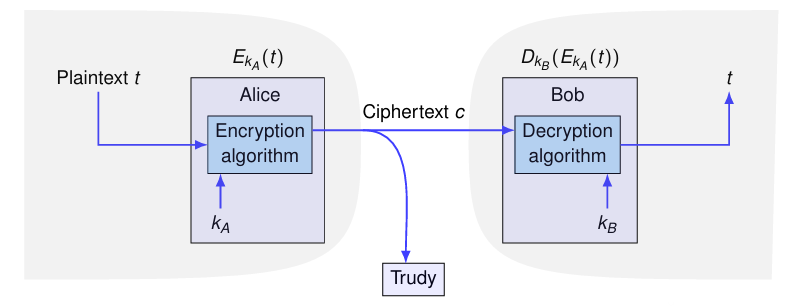
\includegraphics[scale=0.6]{12025-03-18.png}
    \end{center}
   Here Alice want to sent the plaintext $t$ to Bob:
   \begin{itemize}
       \item She encrypts $t$ using her key $k_A$. Theresult is the ciphertext $c = E_{k_A}(t)$
       \item She sends $c$ to Bob over a public channel
       \item Bob decrypts $c$ using his key $k_B$. The result is $D_{k_B}(E_{k_A}(t)) ) t$
       \item For Trudy, it is nearly impossible to recover $t$ from $c$ without knowing $k_B$
   \end{itemize}
\end{parag}
\begin{parag}{Basic Terminology}
    \begin{itemize}
        \item pleintext, ciphertext (also called cryptogram), key, encrypter, decrypter
        \item cryptography: the art of composing cryptograms
        \item cryptanalysis the art of breaking cryptograms
        \item a cryptanalyst has broken the system when he cann quickly determine the plaintext from the cryptogram, no matter what key is used
        \item attacker: same as cryptanalyst
    \end{itemize}

\end{parag}
\begin{parag}{Ancient cryptography}
    \begin{subparag}{Caesar's cipher}
        Suppose that we are using the English alphabet augmented by a few special characters, "space", "comma", and "period".\\ An alphabet of $29$ characters, represented by the integers $0, 1 , \dots, 28$
        \begin{itemize}
            \item The key $k$ is an integer between $0$ and $28$, known to Alice and Bob and to nobody else.
        \item The encryption algorithm substitues the $i$-th letter of the alphabet with the $(i + k)th$ letter $(\mod 29$)
        \item The decryption algorithm substitues the $j$-th letter with the $(j-k)$-th $\mod 29$ 
    \end{itemize}
       Therefore, here the secrecy of the message rely only on the secrecy of the algorithm. 
    \end{subparag}
    \begin{subparag}{Various attacks possible}
        We distinguish between the following attacks:
        \begin{itemize}
            \item \important{ciphertext-only}: one or more cryptograms available to the cryptanalyst know to have been encrypted with the same key
            \item \important{known plaintext}: the cryptanalyst has one or more plaintext and the resulting cryptograms, know to have been encrypted with the same key
            \item \important{chosen plaintext} for any plaintext that he requires, the cryptanalyst can obtain the cryptogram under the same key
        \end{itemize}
        Ideally, a cryptographic system should be secure against a chosen plaintext attack, At the very least, it should be secure against a cipthertext-only attack.
    \end{subparag}
    However with a computer, the key can easily be found using the letter-frequency attack. The question now is how to make the letter frequency attack unfruitful?
\begin{subparag}{Example (Vigenère's cipher with an $n$-length key}
    \begin{itemize}
        \item Chosen plaintext attack: encode the same letter until you have the $n-$length key
        \item \important{known plaintext attack} compare input/output until you have the $n$-length key
        \item \important{ciphertext-only attack}
            \begin{itemize}
                \item brute force approach: try all $29^n$ keys is you know $n$
                    \begin{itemize}
                        \item for $n = 21$ the number of key is $5.13^{30}$
                        \item for $n = 100$, the number of keys is $1.73^{146}$
                    \end{itemize}
                \item If you know $n$, you can partition input/output into $n$ parts, each of which is a Caesar cipher with its own key
                \item Letter frequency approach: effective if the plaintext-length to key-length ration is sufficiently large
            \end{itemize}
    \end{itemize}
\end{subparag}
\end{parag}

\begin{parag}{The one-time pad}
    Preliminary assumptions
    \begin{itemize}
        \item The plaintext $t$, the key $k$ and the cryptogram $c$ are n-length binary sequences over the alphabet $ \mathcal{A} = \{0, 1\}$
        \item The key $k$, is produced by selecting each bit independently and with uniform distribution
        \item Alice and Bob use a private chanel to exchange the key ahead of time
    \end{itemize}
    \textbf{Encryption}
    \begin{align*}
        c = t \oplus k
    \end{align*}
    \textbf{Decryption}
    \begin{align*}
        c \oplus k = (t \oplus k) \oplus k = t \oplus ( k \oplus k) = t
    \end{align*}
    
    

\end{parag}



\begin{parag}{Perfect secrecy}
    \begin{definition}
        A cryptosystem has \important{perfect secrecy} if the plaintext $T$ and the cryptogram $C$ are statistically independent
    \end{definition}
    Perfect secrecy is the ultimate kind of security against a ciphertext-only attack: The attacker cannot do better than guessing the plaintext $T$

\end{parag}
\begin{parag}{Perfect secrecy of the one time pad}
    \begin{itemize}
        \item The $n$-length key $k$ is selected at random (uniform distribution ober $\{0,1\}^n$)
        \item The key $k$ and the message $t$ are selected independently
        \item The ciphertext is $c = t \oplus k$
           \begin{align*}
               p_{C \mid  T}( c \mid  t) = p_{K \mid  T}( c \ominus t \mid  t) = p_K ( c \ominus t ) = \frac{1}{2^n}
           \end{align*}
    \end{itemize}
    Hence $C$ and $T$ are independent: knowledge of $C$ is useless in guessing $T$
\end{parag}
\begin{parag}{Weakness of the one time pad}
    \begin{subparag}{Example}
        A cryptanalyst that has the plaintext $t$ and the corresponding cryptogram $c$ immediately gets the key:
        \begin{align*}
            k = c \ominus t
        \end{align*}
        Hence the pad (the key) should be used only once
    \end{subparag}
    \begin{subparag}{Pros and Cons of one time pad}
        \textbf{Pros}
        \begin{itemize}
            \item Very simple algorithm
            \item as secure as it gets against a ciphertext-only attack and key used one
            \item of instructional value to prove that the perfect secrecy is possible
        \end{itemize}
        \textbf{Cons}
        \begin{itemize}
            \item The key is as long as the plaintext (this is fundamental, see later)
            \item The key needs to be exchanged ahead of time over a private chanel
            \item a ciphertext-only attack can break the system if the key is used twice (see homework)
            \item a known plaintext attack reveals the key
        \end{itemize}
        The "one-time pad" has been used extensively in diplomatic and espionage circles
        
    \end{subparag}

\end{parag}
\begin{parag}{Perfect secrecy requires high entropy keys}
    The following theorem makes no assumption on the encryption algorithm:
    \begin{center}
        \begin{tikzpicture}
            \draw[](0, 0) rectangle(2, 3);
        \draw[<-](2, 2) -- (2.5, 2) node at (2.75, 2) {$t$};
        \draw[->](2, 0.5) -- (2.5, 0.5) node at (2.75, 0.5){$c$};
        \draw[->](-0.5, 1.5) -- (-0, 1.5) node at(-0.75, 1.5){$k$};
        \end{tikzpicture}
        
        
    \end{center}
    
    \begin{theoreme}
        Perfect secrecy implies:
        \begin{align*}
            H(T) \leq H(K)
        \end{align*}
        
    \end{theoreme}
   \begin{subparag}{Proof}
       Perfect secrecy $H(T) = H(T \mid  C)$ and decodability $(H(T \mid  K, C) = 0)$ imply:
       \begin{align*}
           H(T) &= H(T \mid  C)\\
                &\leq H(T, K \mid C)\\
                &= H(K \mid  C) + H(T \mid  K, C)\\
                H(K \mid  C)\\
                &\leq H(K)
       \end{align*}
   \end{subparag}
   \begin{framedremark}
       Entropy plays a key role also in cryptography
   \end{framedremark}
   
\end{parag}



\lecture{10}{2025-03-19}{Encryption?}{}
\begin{parag}{Exercice}
    Determine the minimum average length of the binary key for a cryptosystem that has the following characteristics
\begin{itemize}
    \item the message is an uncompressible binary string of length $n$
    \item the system achieves perfect secrecy
\end{itemize}
\begin{subparag}{Solution}
    \begin{itemize}
        \item $H(T)$ must be essentially $n$ bits (otherwise further compression is possible
        \item Perfect secrecy requires $H(T) \leq H(K)$
        \item  hence $H(K)$ is at least $n$
        \item The average blocklength of the binary key is at least $n$ bits
    \end{itemize}
\end{subparag}
\end{parag}



\begin{parag}{Symettric-Key crypto Systems: key-distribution problem}
         A symmetric-key cryptosystem is one for which both ends use the same key $(k_A = k_B=k)$. All example considered so fare rely on a symmetric key\\
         There exists fast (ans secure) symmetric key cryptosystems, but:
         \begin{itemize}
             \item Anybody that has the key can encrypt and/or decrypt
             \item The key cannot be sent over an insecure channel
             \item In an $n$ user network, each user needs $n-1$ keys to communicate privately with every other user. Key distribution is a problem as it hat to be done over a secure channel. And keys have to be changed frequently
             \item We have a real problem (the first $6$min. and $20$ secs of:
                 \begin{center}
                 \url{https://www.youtube.com/watch?v=YEBfamv-_do}
                 \end{center}
                 
                 
         \end{itemize}
         However, is there a way to distribute keys over a pubic channel?
\end{parag}
\begin{parag}{Solution}
    In 1976, Diffie and Hellman came up with a solution.
    \begin{subparag}{Example}
        You pick a number $p = 7$ which is a prime $ \mathcal{A} = \{0, 1,2 , 3, 4, 5, 6\}$. We then take $ g = 3$
        \begin{center}
           
        \begin{tabular}{cc}
            $i$ & $g^i \mod 7$ \\
            0  & \\
            1 & 3 \\
            2 & 2\\
            3 & 6\\
            4 & 4\\
            5 & 5\\
            6 & 1
        \end{tabular}
        \end{center}
        The gives us a permutation. We have to be careful with choosing the $g$ because for example if we take $g = 2$, and take $g^1$ and $g^4$ the result is $2$ which leads that we don't have a permutations
        
    \end{subparag}
How does it is seen:
\begin{center}
    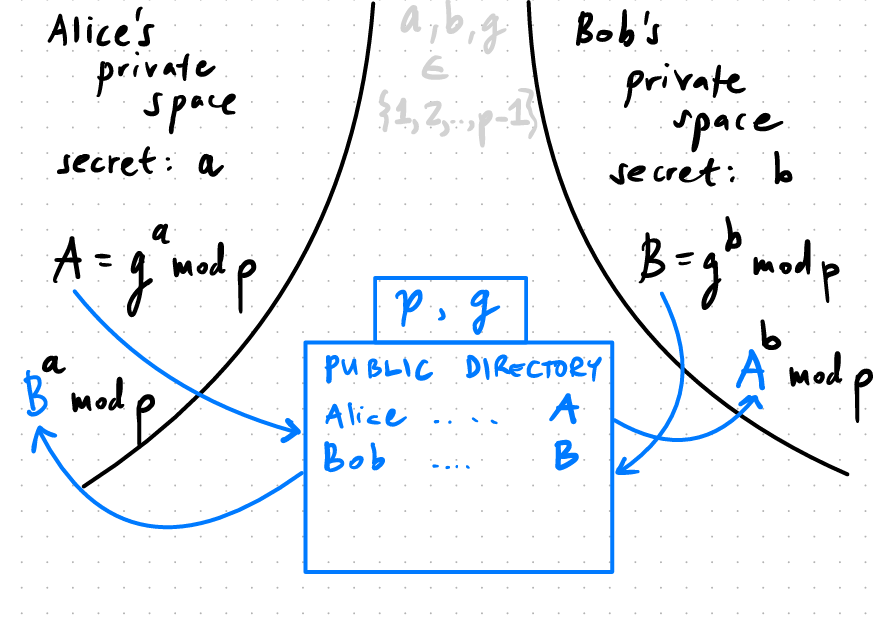
\includegraphics[scale=0.4]{12025-03-19.png}
\end{center}
We have a public directory like a phone book where everyone has access. Alice pick a random $a$. Then she takes a public $A = g^a \mod p$ which we will be written in the public directory. Then Bob do the same thing.  \\
When Alice and Bob want to have an interaction. Alice will look for Bob in the phonebook, take the $B$ in her private space, take the result of $B^a \mod p$ (she is the only one to know $a$). Bob do the same thing: $A^b \mod p$\\
\textbf{At this point} 
\begin{itemize}
    \item Alice has  $B^a \mod p$
        \begin{align*}
            B^a = (g^b \mod p)^a \mod p
        \end{align*}
    \item Bob has $A^b \mod p$
        \begin{align*}
            A^b = (g^a \mod p)^b \mod p
        \end{align*}
        
        
       
\end{itemize}
\begin{subparag}{Fact}
    \begin{theoreme}
        For all $x, y, m \in \mathbb{Z}$:
        \begin{align*}
            \left[ (x \mod m) \cdot (y \mod m) \right] \mod m = xy \mod m
        \end{align*}
        
    \end{theoreme}
    We then get $B^a = g^{ab} \mod p$ and $A^b = g^{ab} \mod p$ We juste need to find the inverse of $g^i \mod p$ Which is a discrete logarithm problem. It is very hard to find the discrete logarithm. The gives the secrecy of this encryption. The secrecy is only here because it is hard to compute this inverse

\end{subparag}
\begin{subparag}{Secrecy}
    But can't anybody generate this key?\\
    We all know $g$ and we know that $A = g^a \mod p$ we juste has to find
    
\end{subparag}
\begin{subparag}{Eve wants to listen}
    Assuming that the cryptosystem used by Bob and Alise is secure, the best option for Eve is to find the key $k$. \\
    She know $p, g, A$ and $B$.\\
    In generale, there seems to be no better way than finding the number $a$ for which $g^a = A$, and the comput $k = B^a$\\
    This is a problem. Let us check out some number. Suppose $p$ is a 2048 bit number. (it must be prime, but let us neglect this and assume $p  = 2^{2048}$ How long does it take to compute:
    \begin{align*}
        2\log_2 p = 4096
    \end{align*}
    Multiplications to performs $a \to g^a$ (called discrete exponentiation). With a computer that performs $10^{10}$ multiplications per seconds, the exponentiation is done seamlessly.\\
    It takes roughly:
    \begin{align*}
        \text{exp} \left( \left( \frac{64}{9} \right)^{ \frac{1}{3}} (\ln p)^{ \frac{1}{3}} \ln \ln p)^{ \frac{2}{3}} \right) \approx 10^{35}
    \end{align*}
    Mutliplication to perform $g^a \to a$ (called discrete logarithm to the base $g$. With the same computer, it takes about $10^{25}$ seconds, which is about $7 \cdot 10^{7}$ times the ages of the earth.
\end{subparag}
\begin{subparag}{Conclusion}
    Diffie and Hellman's public key distribution scheme is clever, efficient, and it seems to be secure.
\end{subparag}
\end{parag}

\begin{parag}{Paradigm shift}
    The issue with the security is the computation. For example in maybe a couple of years the quantum computer will be able to compute this discrete algorithm very fast. The DG system would instanlty become insecure.\\
    To the constrast, perfect secrecy offers provable security even when the enemy has infinite time and computing power. Most cryptographic systems rely on computational security


\end{parag}
\begin{parag}{One way function}
    Discrete exponentiation is an example of a one  way function: a function for which a fast algorithm exists one way but not in the other way. The case for the discrete logarithm is that there is a way back but it is very slow. However, the best case would be that there is not way back.
    \begin{subparag}{Example}
        IF a computer were to save user's names and passwords, a sstem manager would have access to both.\\
        This is not the case if the operating system stores, along the name a one-way function $f$ of our password.( The password itself is never stored)
        
    \end{subparag}
    
\end{parag}

\begin{parag}{Trapdoor One-way function}
    A tropdoor one way function is a one-way function with an extra feature called the trapdoor information: with this information, the hard-to-carry out inverse computation becomes easy.\\
    Diffie and Hellmann realized that with such a tool the key distribution problem would diseappear

\end{parag}



\begin{parag}{Asymetric cryptography}
    Suppose that Allice wants to send private information to Bob\\
        Bob has a trapdoor one-way function, implemented by an algorithm $E_B$ that he publsishes in a open directory\\
        He is the only one who has the trapdoor information $k_B$. Hence he has the algorithm $D_B$ that implements the inverse function.\\
        Alice and Bob no longer need a shared key:
        \begin{center}
           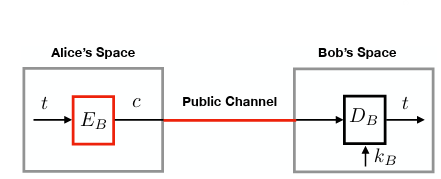
\includegraphics[scale=0.8]{22025-03-19.png} 
        \end{center}

\end{parag}
\begin{parag}{ElGammal's trapdoor one way function}
    \begin{subparag}{Setup}
        \begin{itemize}
            \item Fix a large prime number $p$. Hereafter all the numbers are in $\{0, 1, \dots, p1\}$ and arithmetic is modulo $p$ (mor on it later).
            \item Pick a generator $g$
            \item Pick randomly selected numbers $x$ and $y$. Unlike $p$ and $g$,$x$, and $y$ are kept secret.\\
            \item  Here is a trapdoor one-way function, with \important{trapdoor information} $x$.
                \begin{center}
                    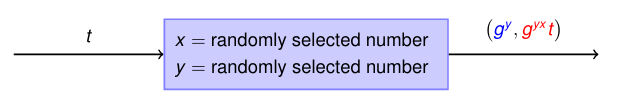
\includegraphics[scale=0.5]{32025-03-19.png}
                \end{center}
        \end{itemize}
        
        Given the trapdoor information $x$, we can invert the function as follows:
        Compute the inverse of $g(^y)^x = g^{xy}$, multiply the result with $g^{xy}t$. The result is $t$.
    \end{subparag}
\begin{subparag}{More concretly}
    Alice has:
    \begin{itemize}
        \item $t$ = plaintex, $t$
        \item $y = $ random number, $y$
    \end{itemize}
    Bob:
    \begin{itemize}
        \item $x$ = random number $x$.
    \end{itemize}
    The scheme look like this:
    \begin{center}
        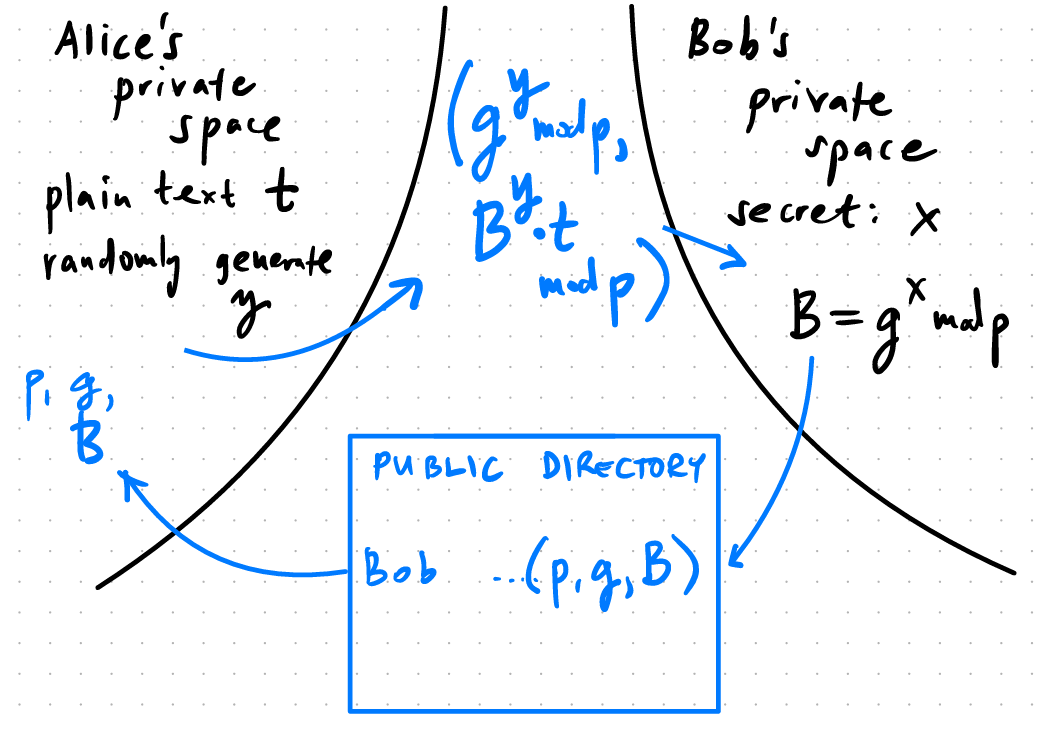
\includegraphics[scale=0.5]{42025-03-19.png}
    \end{center}
    Bob sends $g^x$ to Alice, then Alice sends the cryptogram $(g^y, g^{xy}t)$ to Bob
    \begin{framedremark}
        Note: $x$ and $y$ are transaction specific
    \end{framedremark}
    
    
    
\end{subparag}
\end{parag}



\end{document}
